\chapter{Results} 
\label{chapter:results}

In this chapter, we sum up the results of the research of this thesis. We illustrate the key insights and challenges faced in answering each research question. To obtain our results, we followed the methodology formulated in \autoref{chapter:method}.


\section{\rqone}
\label{results:rq1}


\newcommand{\rossetapopulationunique}{2678}
\newcommand{\rossetapopulation}{809900}
\newcommand{\diversifiedsodium}{85}
\newcommand{\diversifiedqrcode}{32}
\newcommand{\libsodiumpopulation}{4272}
\newcommand{\libsodiumpopulationunique}{3805}
\newcommand{\qrpopulation}{6369}
\newcommand{\qrpopulationunique}{3314}


\newcommand{\allmewediversified}{\diversifiedsodium + \diversifiedqrcode}
\newcommand{\allmewepopulation}{\libpopulation + \qrpopulation}

As we describe in \autoref{rq1:method}, our first research question aims to answer how to artificially generate \wasm program variants. 
This section is organized as follows. First we present the general results calculating the \emph{\corpuspopulationsizename}(\autoref{metric:rq1:corpus_pop}) and \emph{\corpusuniquepopulationsizename}(\autoref{metric:rq1:corpus_pop_unique}) for each corpus. 
Second, we discuss the challenges and limitations in program variants generation. Finally, we illustrate the most common code transformations performed by our approach and answer RQ1.

\subsection{Program's population}

We summarize the results in \autoref{table:crow:general_results}.
The table illustrates the corpus name, the number of functions to diversify, the number of successfully diversified functions (functions with at least one artificially created variant), the cumulative number of variants (\emph{\corpuspopulationsizename}) and the cumulative number of unique variants (\emph{\corpusuniquepopulationsizename}).

% General results on the number of diversified functions per corpus
We produce at least one unique program variant  for $239/303{}$ single function programs for \corpusrosetta with one hour for a diversification timeout. For the rest of the programs ($64/303{}$), the timeout is reached before CROW can find any valid variant. 
In the case of \corpussodium and \corpusqrcode, we produce variants for $\pypy{\diversifiedsodium}/\pypy{\libsodiumfunctions}$ and $\pypy{\diversifiedqrcode}/\pypy{\qrcodefunctions}$ functions respectively, with 5 minutes per function as timeout. The rest of the functions resulted in timeout before finding function variants or produce no variants. For all programs in all corpora, we achieve $356/3021$ successfully diversified functions, representing a $11.78\%$ of the total.
% General growing factor
As the four and fifth columns show, the number of artificially created variants and the number of unique variants are larger than the original number of functions by one order of magnitude. In the case of \corpusrosetta, the corpus population size is close to one million of programs.
The remarkable difference between the total number of variants and the number of unique variants (fourth and fifth columns) is mainly due to the \emph{replacements combining} process discussed in \autoref{section:crow}.

%\todo{M: Elaborate on uniqueness...}

% \todo{M: add histogram on variant sizes}

{
    \renewcommand{\arraystretch}{1.6}
\begin{table}[h]
    %\small
    \centering
    %\setlength\minrowclearance{1.0pt}
        \begin{tabular}[t]{ l | r | l  | l | r}
     Corpus & \#Functions & \# Diversified &  \# Variants & \#  Unique  Variants \\
        \hline   

        \corpusrosetta & \fromjson{data/crow_corpus.json}{.[0].functions} & 239 & \rossetapopulation  &  \rossetapopulationunique \\
        \hline


        \corpussodium & \libsodiumfunctions & \diversifiedsodium & \libsodiumpopulation & \libsodiumpopulationunique     \\
        \hline

        \corpusqrcode & \qrcodefunctions & \diversifiedqrcode  &  \qrpopulation & \qrpopulationunique \\

        \hline\hline

         & \pypy{\libsodiumfunctions + \qrcodefunctions + 303 } & \pypy{239 + \diversifiedqrcode +\diversifiedsodium}  & \pypy{\qrpopulation + \rossetapopulation + \libsodiumpopulation} & \pypy{\qrpopulationunique + \rossetapopulationunique + \libsodiumpopulationunique}   \\
        \end{tabular}
    
        \caption{General program's populations statistics. The table is composed by the name of the corpus, the number of functions, the number of succesfully diversified functions, the cumulative number of generated variants and the cumulative number of unique variants.}
        \label{table:crow:general_results}
\end{table}
}


\subsection{Challenges for automatic diversification}
\label{rq1:challenges}

% Low diversified functions
We have observed a noticeable difference between the number of successfully diversified functions versus the number of failed-to-diversify functions (third column of \autoref{table:crow:general_results}). Our approach successfully diversified $239/303$, $85/869$ and $32/1849$ of the original functions for \corpusrosetta, \corpussodium and \corpusqrcode respectively.  %The main reason of this phenomenon is the set timeout for CROW. 
%\todo{so what? what does this mean for practitioners?: Setting up the timeout affects the capacity of our approach to generate variants. For our corpora, a low timeout implies a low number of diversified functions.}

% High populatio size
We have noticed a remarkable difference between the number of diversified functions for each corpus, \rossetapopulation\ programs for \corpusrosetta 4272 for \corpussodium and 6369 for \corpusqrcode. The corpus population size for \corpusrosetta is two orders of magnitude larger compared to the other two corpora. The reason behind the large number of variants for \corpusrosetta is that, after certain time, our approach starts to combine the code replacements to generate new variants. However, looking at the fifth column, the number of unique variants have the same order of magnitude for all corpora.
The variants generated out of the combination of several code replacements are not necessarily unique. Some code replacements can dominate over others, generating the same \wasm programs.

% Why large unique count in low time ? 
A low timeout offers more unique variants compared to the population size despite the low number of diversified functions, like the \corpussodium and \corpusqrcode cases. This happens because, CROW first generates variants out of single code replacements and then starts to combine them. Thus, more unique variants are generated in the very first moments of the diversification process with CROW.

%Moreover, we look at the cases that yield a few variants per function. There is no direct correlation between the number of identified codes for replacement and the number of unique variants. Therefore, 

Apart from the timeout and the combination of variants phenomenon, we manually analyze programs, searching for properties attempting to the generation of program variants using CROW.
As we previously mentioned in \autoref{section:crow}, \emph{constant inferring} is a new contribution of ours to the collection of Software Diversification strategies enumerated in \autoref{sota:sota}. 
We have observed that our approach searches for a constant inferring for more than $45\%$ of the instructions of each function while constant values cannot be inferred in all cases. The main reason is that memory operations are also included into the inferring while our tool is oblivious to a memory model, making unsuccessful the constant replacement.

\subsection{Properties for large diversification}

We manually analyzed the programs to study the critical properties of programs producing a high number of variants.
This reveals one key factor that favors many unique variants: the presence of bounded loops. In these cases, we synthesize variants for the loops by replacing them with a constant, if the constant inferring is successful. Every time a loop constant is inferred, the loop body is replaced by a single instruction. This creates a new, statically different program. The number of variants grows exponentially if the function contains nested loops for which we can successfully infer constants. 

A second key factor for synthesizing many variants relates to the presence of arithmetic expressions. The synthesis engine used by our approach, effectively replaces arithmetic instructions with equivalent instructions that lead to the same result. For example, we generate unique variants by replacing multiplications with additions or shift left instructions (\autoref{add:example}). Also, logical comparisons are replaced, inverting the operation and the operands (\autoref{cmp:examples}). Besides, our implementation can use overflow and underflow of integers to produce variants (\autoref{overflow:example}).

{
\begin{code}
    \footnotesize
    \lstdefinestyle{nccode}{
        numbers=none,
        firstnumber=2,
        stepnumber=1,
        numbersep=10pt,
        tabsize=4, 
        showspaces=false,
        breaklines=true, 
        showstringspaces=false,
        moredelim=**[is][\btHL]{`}{`},
        moredelim=**[is][{\btHL[fill=black!10]}]{`}{`},
        moredelim=**[is][{\btHL[fill=celadon!40]}]{!}{!}
    }

    \lstset{
        language=WAT,
        style=nccode,
        basicstyle=\footnotesize\ttfamily,
        columns=fullflexible,
        breaklines=true
    }
    \noindent\begin{minipage}[b]{0.32\linewidth}
        \captionof{lstlisting}{Diversification through arithmetic expression replacement.}\label{add:example}
        \noindent\begin{minipage}[t]{0.46\linewidth}
            \begin{lstlisting}
local.get 0
`i32.const 2`
`i32.mul`
            \end{lstlisting}
        \end{minipage}%
        \hfill\noindent\begin{minipage}[t]{0.46\linewidth}
            
            \begin{lstlisting}
local.get 0
!i32.const 1!
!i32.shl!
            \end{lstlisting}
        \end{minipage}
    \end{minipage}\hfill%
    \begin{minipage}[b]{0.31\linewidth}
        \captionof{lstlisting}{Diversification through inversion of comparison operations.}\label{cmp:examples}
        \begin{minipage}[t]{.46\linewidth}
            \begin{lstlisting}
`local.get 0`
`i32.const 10`
`i32.gt_s`
            \end{lstlisting}
        \end{minipage}\hfill\begin{minipage}[t]{.46\linewidth}
           
            \begin{lstlisting}
!i32.const 11!
!local.get 0!
!i32.le_s!
            \end{lstlisting}
        \end{minipage}%
        
        
    \end{minipage}\hfill\noindent
    \noindent\begin{minipage}[b]{0.32\linewidth}
        \captionof{lstlisting}{Diversification through overflow of integer operands.}\label{overflow:example}
        \noindent\begin{minipage}[t]{0.46\linewidth}
            \begin{lstlisting}
`i32.const 2`
i32.mul
\end{lstlisting}
        \end{minipage}%
        \hfill\noindent\begin{minipage}[t]{0.46\linewidth}
            
            \begin{lstlisting}
i32.const 2
i32.mul
!i32.const!
!  -2147483647!
!i32.mul!
            \end{lstlisting}
        \end{minipage}
    \end{minipage}
    \end{code}
}

At the \wasm level, we have not observed variants performing changes in the control flow structure of the program (\autoref{strategy:S3}). 
Yet, this is not the case when we manually analyze the machine code generated by V8 (as it was discussed in \autoref{sota:wasm}).
For the generated machine code, we have observed that, for different variants, we are changing the number of jumps and its locations.
The control flow change strategy (\autoref{strategy:S3}) is correctly achieved as a consequence of latter compilation of Wasm program variants.
%This fact encourages us for future work on the impact of our Software Diversification technique in the latest stage of \wasm program generation, machine code.

\begin{tcolorbox}[title=Answer to RQ1.,boxrule=2pt,arc=.3em,boxsep=1.5mm]
    We can provide diversification for 11.78\% of the programs in our corpora. Constant inferring, complemented with the high presence of arithmetic operations and bounded loops in the original program increased the number of program variants. 
    %\todo{Remove or elaborate: Nevertheless, the combination of code replacements in our approach is not a determinant factor to provide a large number unique program variants.}
\end{tcolorbox}



\begin{comment}

While our work is very limited by the provided corpora, it can be easily extended to other\dots

An application that benefits from the ablity of CROW is the large amount of generated variants. 


- CHeckLong questions for 80%
- Stress how to do experiments in Software Engineering, the theory behind how to do this in CS.
- The objects of the experiments are programs that ... 
- Motivate the corpora selection, size, can be ported, security sensitive, etc,
- Do not mention CROW in the selection criteria.
- The motivation is not related to tools, only to concepts
- Move paragraph after listing of coprpora to before.
- 
%The proposed methodology can generate program variants that are syntactically different from their original versions. We have shown that CROW generates diversity among the binary code variants using semantically equivalent code transformations. We identified the properties that original programs should have to provide a handful number of variants. Besides, we enumerated the challenges faced to provide automatic diversification by retargeting a superoptimizer.

%In the next chapter, we evaluate the assessment of the generated variants answering to what extent the artificial programs are different from the original in terms of static difference, execution behavior, and preservation.

\end{comment}

\section{\rqtwo}



Our second research question investigates the differences between program variants at runtime.
To answer RQ2, we execute each program/variant generated to answer RQ1 for \corpusrosetta corpus to collect their execution traces and execution times.
For each programs' population we compare the stack operation traces (\autoref{metric:stack}) and the execution-time distributions (\autoref{metric:time}) for each program/variant pair.

This section is organized as follows. First, we analyze the programs' populations by comparing the traces for each pair of program/variant with \DTW of \autoref{metric:stack}. The pairwise comparison will hint at the results at the population level. We analyze not only the differences of a variant regarding its original program, we also compare the variants against other variants. Second, we do the same pairwise strategy for the execution-time distributions \autoref{metric:time}, performing a Mann-Withney U test for each pair of program/variant times distribution. Finally, we conclude and answer RQ2.

\subsection{Stack operation traces.}


% Describe the first figure
In \autoref{rq2:dtw_distrib} we plot the distribution of all comparisons (in logarithmic scale) of all pairs of program/variant in each programs' population. All compared programs are statically different. Each vertical group of blue dots  represents all the pairwise comparison of the traces (\autoref{metric:stack}) for a program of the \corpusrosetta corpus for which we generate variants.
Each dot represents a comparison between two programs' traces according to \autoref{metric:stack}. 
The programs are sorted by their number of variants in descending order. For the sake of illustration, we filter out those programs for which we generate only 2 unique variants. 

\begin{figure}[h]
    \centering
    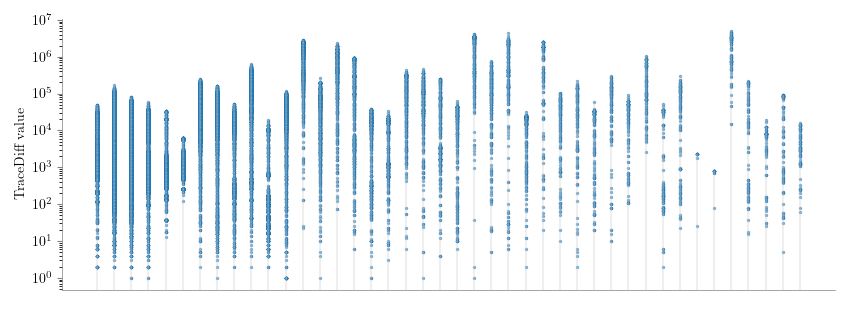
\includegraphics[width=\linewidth]{plots/plot_distribs1.png}
    \caption{Pairwise comparison of programs' population traces in logarithmic scale. Each vertical group of blue dots represents a programs' population. Each dot represents a comparison between two program execution traces according to \autoref{metric:stack}. }
    \label{rq2:dtw_distrib}
\end{figure}

% Main insight
We have observed that in the majority of the cases, the mean of the comparison values is remarkably large. We analyze the length of the traces, and one reason behind such large values of \DTW is that some variants result from constant inferring. For example, if a loop is replaced by a constant, instead of several symbols in the stack operation trace, we observe one. Consequently, the distance between two program traces is significant. 

% What happens with programs with the same trace ?
In some cases, we have observed variants that are statically different for which \DTW value is zero, \ie they result in the same stack operation trace. We identified two main reasons behind this phenomenon. First, the code transformation that generates the variant targets a non-executed or dead code. Second, some variants have two different instructions that trigger the same stack operations. For example, the code replacements below illustrate the case. 

\begin{code}[H]
\centering
\noindent\begin{minipage}{.23\linewidth}
\lstdefinestyle{nccode2}{
    numbers=none,
    firstnumber=1,
    stepnumber=1,
    numbersep=10pt,
    tabsize=4,
    showspaces=false,
    breaklines=true, 
    showstringspaces=false,
    moredelim=**[is][{\btHL[fill=black!10]}]{`}{`},
    moredelim=**[is][{\btHL[fill=celadon!40]}]{!}{!}
}
    \lstset{
        language=WAT,
        style=nccode2,
        basicstyle=\footnotesize\ttfamily,
        columns=fullflexible,
        breaklines=true
    }
    \begin{lstlisting}
(1) `i32.lt_u`
(2) `i32.le_s`
    \end{lstlisting}
\end{minipage}\hfill%
\noindent\begin{minipage}{0.2\linewidth}
\lstdefinestyle{nccode2}{
    numbers=none,
    firstnumber=1,
    stepnumber=1,
    numbersep=10pt,
    tabsize=4,
    showspaces=false,
    breaklines=true, 
    showstringspaces=false,
    moredelim=**[is][{\btHL[fill=black!10]}]{`}{`},
    moredelim=**[is][{\btHL[fill=celadon!40]}]{!}{!}
}

    \lstset{
        language=WAT,
        style=nccode2,
        basicstyle=\footnotesize\ttfamily,
        columns=fullflexible,
        breaklines=true
    }
    \begin{lstlisting}
!i32.lt_s!
!i32.lt_u!
    \end{lstlisting}
\end{minipage}\hfill%
\noindent\begin{minipage}{.3\linewidth}
\lstdefinestyle{nccode2}{
    numbers=none,
    firstnumber=1,
    stepnumber=1,
    numbersep=10pt,
    tabsize=4,
    showspaces=false,
    breaklines=true, 
    showstringspaces=false,
    moredelim=**[is][{\btHL[fill=black!10]}]{`}{`},
    moredelim=**[is][{\btHL[fill=celadon!40]}]{!}{!}
}

    \lstset{
        language=WAT,
        style=nccode2,
        basicstyle=\footnotesize\ttfamily,
        columns=fullflexible,
        breaklines=true
    }
    \begin{lstlisting}
(3) `i32.ne`
(4) `local.get 6`
    \end{lstlisting}
\end{minipage}\hfill%
\noindent\begin{minipage}{0.2\linewidth}
\lstdefinestyle{nccode2}{
    numbers=none,
    firstnumber=1,
    stepnumber=1,
    numbersep=10pt,
    tabsize=4,
    showspaces=false,
    breaklines=true, 
    showstringspaces=false,
    moredelim=**[is][{\btHL[fill=black!10]}]{`}{`},
    moredelim=**[is][{\btHL[fill=celadon!40]}]{!}{!}
}

    \lstset{
        language=WAT,
        style=nccode2,
        basicstyle=\footnotesize\ttfamily,
        columns=fullflexible,
        breaklines=true
    }
    \begin{lstlisting}
!i32.lt_u!
!local.get 4!
    \end{lstlisting}
\end{minipage}
\end{code}

In the four cases, the operators are different (original in gray color and the replacement in green color) leaving the same values for equal operands.
The (1) and (2) cases are comparison operations leaving the value $0$ or $1$ in the stack taking into account the sign of their operands.  In the third case, the replacement is less restricted to the original operator, but in both cases, the codes leave the same value in the stack. In the last case, both operands load a value of a local variable in the stack, the index of the local variable is different but the value of the variable that is appended to the trace is the same in both cases. 

\subsection{Execution times.}

%\todo{recall again that execution time diversification is important, should the reader have forgotten about this.}

Even when two programs of the same population offer different execution traces, their execution times can be similar (statistically speaking). In practice, the execution traces of \wasm\ programs are not necessarily accessible, being not the case with the execution time. For example, in our current experimentation we need to use our own instrumentation of the execution engine to collect the stack trace operations while the execution time is naturally accessible in any execution environment. This mentioned reasoning enforces our comparison of the execution times for the generated variants. Besides the execution times of programs can be used by malicious clients to construct personalized attacks \cite{morgan2015web}. Therefore, by measuring the execution times, we assess the diversification of observable behaviors evaluated in real-world security scenarios.


For each program's population, we compare the execution-time distributions, \autoref{metric:time}, of each pair of program/variant.
Overall diversified programs, $169$ out of $239$ ($71\%$) have at least one variant with a different execution-time distribution than the original program (P-value $<$ $0.01$ in the Mann-Withney test). This result shows that we effectively generate variants that yield significantly different execution times.

By analyzing the data, we observe the following trends. First, if our tool infers control-flows as constants in the original program, the variants execute faster than the original, sometimes by one order of magnitude. On the other hand, if the code is augmented with more instructions, the variants tend to run slower than the original. 

In both cases, we generate a variant with a different execution time than the original. Both cases are good from a randomization perspective since this minimizes the certainty a malicious user can have about the program's behavior. Therefore, a deeper analysis of how this phenomenon can be used to enforce security will be discussed in answering RQ3.

To better illustrate the differences between executions times in the variants, we dissect the execution-time distributions for one programs' population of \corpusrosetta. The plots in \autoref{rq3:perf} show the execution-time distributions for the \texttt{Hilbert curve} program and their variants. 
We illustrate time diversification with this program because, we generate unique variants with all types of transformations previously discussed in \autoref{results:rq1}.
In the plots along the X-axis, each vertical set of points represents the distribution of 100000 execution times per program/variant. The Y-axis represents the execution time value in milliseconds. The original program is highlighted in green color: the distribution of 10000 execution times is given on the left-most part of the plot, and its median execution time is represented as a horizontal dashed line. The median execution time is represented as a blue dot for each execution-time distribution, and the vertical gray lines represent the entire distribution. The bolder gray line represents the 75\% interquartile. The program variants are sorted concerning the median execution time in descending order.

\begin{figure*}[h]
    \centering
    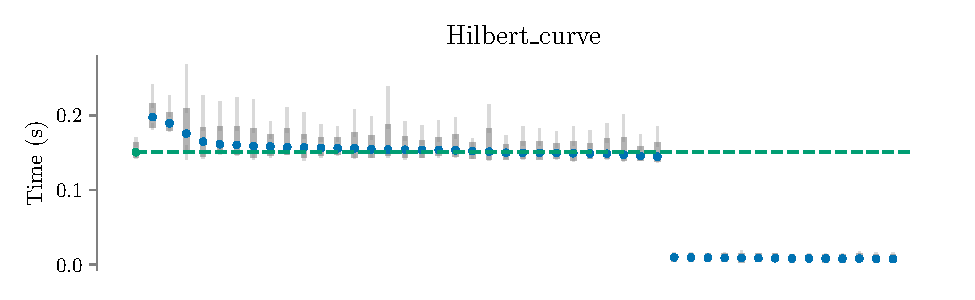
\includegraphics[width=\linewidth]{plots/hilbert_curve.pdf}
    \caption{Execution-time distributions for \texttt{Hilber\_curve} program and its variants. Baseline execution time mean is highlighted with the magenta horizontal line. }
    \label{rq3:perf}
\end{figure*}

% explanation
For the illustrated program, many diversified variants are optimizations (blue dots below the green bar). The last third represents faster variants resulting from code transformations that optimize the original program.
Our tool provides program variants in the whole spectrum of time executions, lower and faster variants than the original program. The developer is in charge of deciding between taking all variants or only the ones providing the same or less execution time for the sake of performance. Nevertheless, this result calls for using this timing spectrum phenomenon to provide binaries with unpredictable execution times by combining variants. The feasibility of this idea will be discussed in \autoref{results:rq3}.


\begin{tcolorbox}[title=Answer to \rqtwo,boxrule=2pt,arc=.3em,boxsep=1.5mm]
    We empirically demonstrate that our approach generates program variants for which execution traces are different. We stress the importance of complementing static and dynamic studies of programs variants. For example, if two programs are statically different, that does not necessarily mean different runtime behavior. There is at least one generated variant for all executed programs that provides a different execution trace. 
    % answer to RQ2
    We generate variants that exhibit a significant diversity of execution times. Concretely, for $169/239\,(71\%)$ of the diversified programs, at least one variant has an execution-time distribution that is different compared to the execution-time distribution of the original program. 
    The result from this study encourages the composition of the variants to provide a resilient execution.
\end{tcolorbox}

\section{\rqthree}
\label{results:rq3}

Here we investigate the impact of the composition of program variants into \termidx[multivariant ]{Software!Multivariant}binaries.
To answer this research question, we create \termidx[multivariant ]{Software!Multivariant}binaries from the program variants generated for \corpussodium and \corpusqrcode corpora. Then, we deploy the \termidx[multivariant ]{Software!Multivariant}binaries into the Edge and collect their execution times. 

\subsection*{Execution times and timing side-channels.}

%\todo{either you call this way in both RQ2 and RQ3 or you don't. but consistently.}

We compare the execution time distributions for each program for the original and the \termidx[multivariant ]{Software!Multivariant}binary. All distributions are measured on 100k executions of the program along all Edge platform nodes.
% statistics
We have observed that the distributions for \termidx[multivariant ]{Software!Multivariant}binaries have a higher standard deviation of execution time.
A statistical comparison between the execution time distributions confirms the significance of this difference (P-value = 0.05 with a  Mann-Withney U test). This hints at the fact that the execution time for \termidx[multivariant ]{Software!Multivariant}binaries is more unpredictable than the time to execute the original binary. 


% Curve flatenning
In \autoref{rq3:diversity:times}, each subplot represents the quantile-quantile plot \cite{gnanadesikan1968probability} of the two distributions, original and \termidx[multivariant ]{Software!Multivariant}binary.
This kind of plots is used to compare the shapes of distributions, providing a graphical comparison of location, scale, and skewness for two distributions.
The dashed line cutting the subplot represents the case in which the two distributions are equal, \ie for two equal distribution we would have all blue dots over the dashed line. These plots reveal that the execution times are different and are spread over a more extensive range of values than the original binary.
The standard deviation of the execution time values evidences the latter, the original binaries have lower values while the \termidx[multivariant ]{Software!Multivariant}binaries have higher values up to $100$ times the original. Besides, this can be graphically appreciated in the plots when the blue dots cross the reference line from the bottom of the dashed line to the top.
This is evidence that execution time is less predictable for \termidx[multivariant ]{Software!Multivariant}binaries than original ones.
This phenomenon is present because the choice of function variants is randomized at each function invocation, and the variants have different execution times due to the code transformations, i.e., some variants execute more instructions than others. 
 

\begin{figure*}[h]
    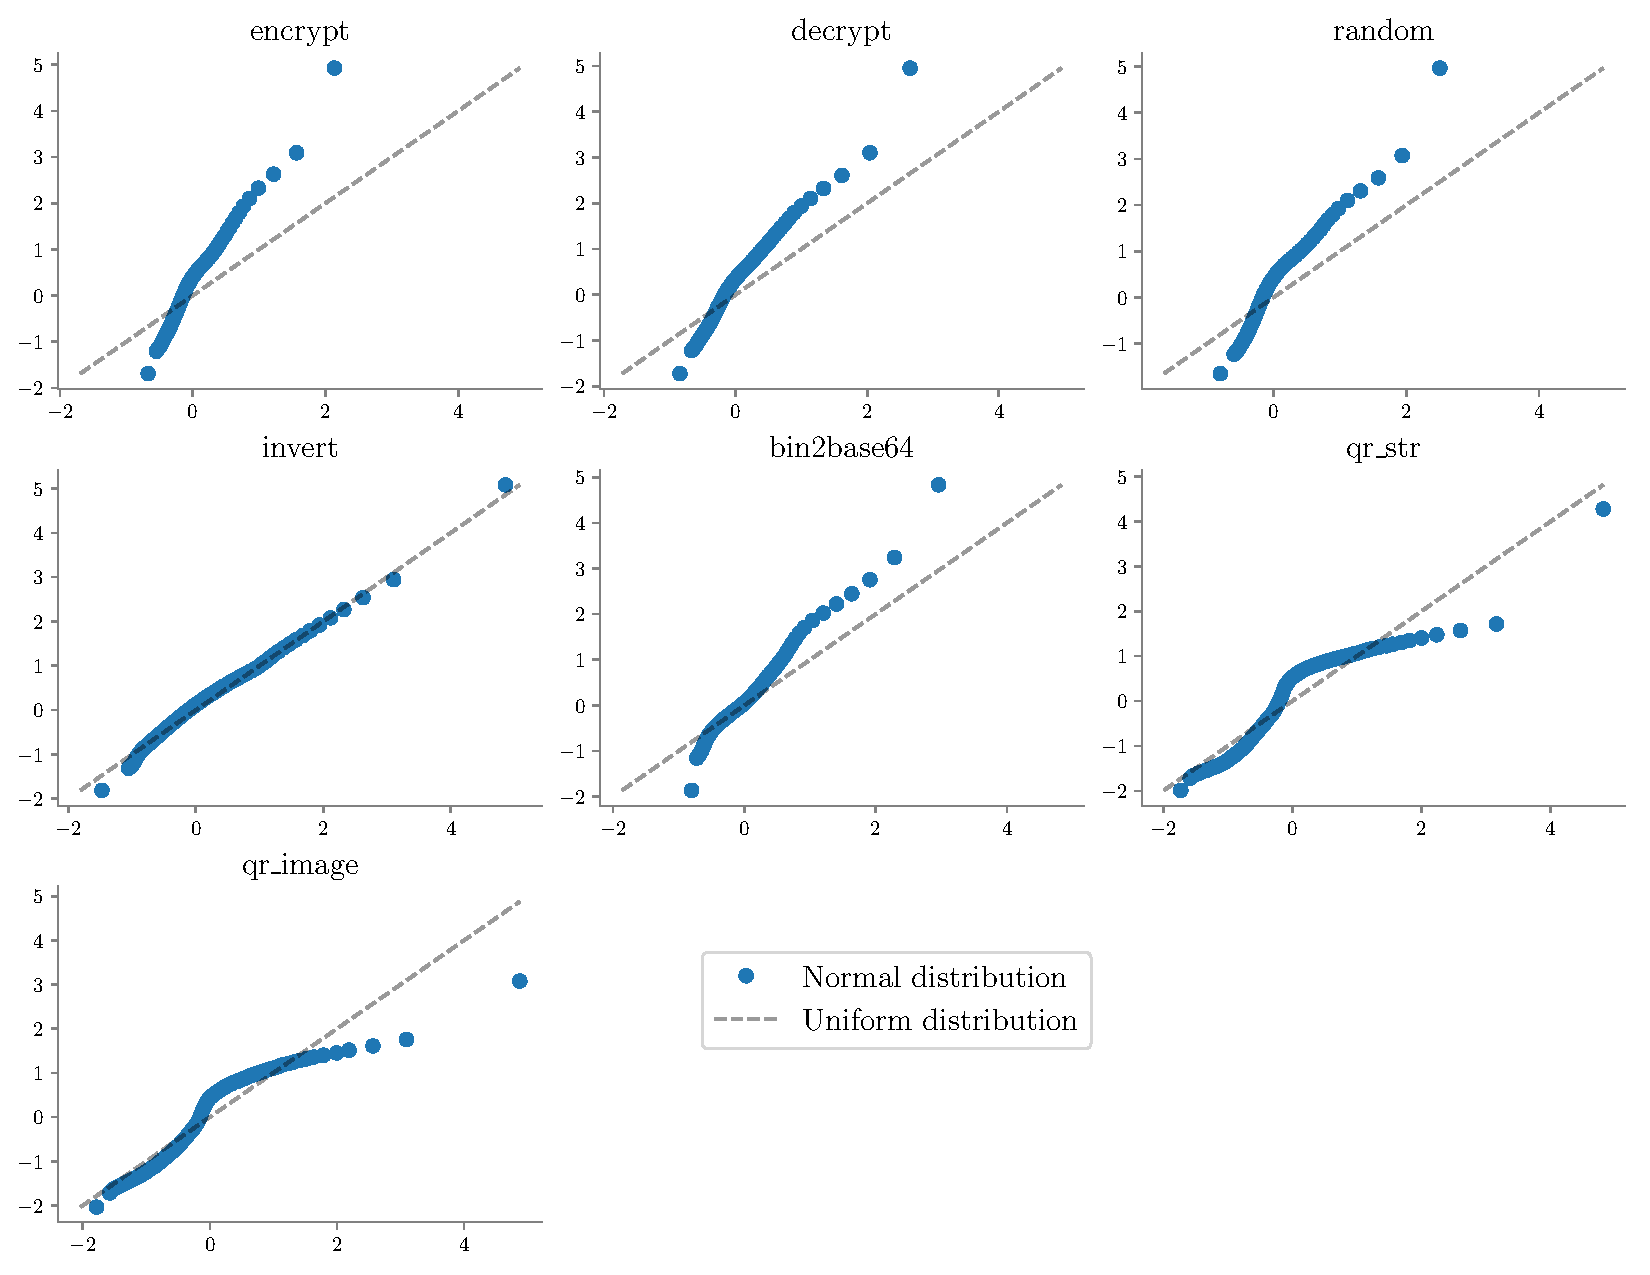
\includegraphics[width=\linewidth]{plots/qqplots.pdf}
    \caption{Execution time distributions. Each subplot represents the quantile-quantile plot of the two distributions, original and \termidx[multivariant ]{Software!Multivariant}binary. }
    \label{rq3:diversity:times}
\end{figure*}



\begin{tcolorbox}[title=Answer to RQ3.,boxrule=2pt,arc=.3em,boxsep=1.5mm]
    
The execution time distributions are significantly different between the original and the \termidx[multivariant ]{Software!Multivariant}binary. Furthermore, no specific variant can be inferred from execution times gathered from the \termidx[multivariant ]{Software!Multivariant}binary. 
Consequently, attacks relying on measuring precise execution times \cite{blackhatpaper} of a function are made a lot harder to conduct as the distribution for the \termidx[multivariant ]{Software!Multivariant}binary is different and even more spread than the original one.

\end{tcolorbox}

% Define some numbers here for the autmation of the tables

%\pagebreak
\section*{Conclusions}

Our approach introduces static and dynamic, variants for up to 11.78\% of the programs in our three corpora, increasing the original count of programs by $4.15$ times. We highlighted the importance of complementing static and dynamic studies for programs diversification. Moreover, combining function variants in multivariant binaries makes virtually impossible to predict which variant is executed for a given query. We empirically demonstrate the feasibility and the application of automatically generating \wasm program variants.

% While our approach targets \wasm environments, previous works have demonstrated the importance of execution path randomization \cite{davi2015isomeron}. The work of Davi \etal proposed to randomly switch between two program executions, the original and a variant to provide an unpredictable behavior. 
